\begin{frame}{Kodierer Information}

\begin{itemize}
\tightlist
\item
  Nicht-Rekursiver Kodierer
\item
  Anzahl von Ausgängen : \[N=2\]
\item
  Anzahl von Registern : \[M=2\]
\item
  Generatoren : \[(7,5)_8 = \begin{pmatrix}111 \\ 101 \\ \end{pmatrix}\]
\item
  Kode-Rate: \[\frac{1}{2}\]
\end{itemize}

\end{frame}

\begin{frame}[fragile]{Kodierer Matrix : Nächster Zustand}

\begin{Shaded}
\begin{Highlighting}[]
\NormalTok{next.table <-}\StringTok{ }\NormalTok{next.state}
\KeywordTok{colnames}\NormalTok{(next.table) <-}\StringTok{ }\KeywordTok{c}\NormalTok{(}\StringTok{"Bit 0"}\NormalTok{, }\StringTok{"Bit 1"}\NormalTok{)}
\NormalTok{row.counter <-}\StringTok{ }\KeywordTok{rep}\NormalTok{(}\DecValTok{1}\NormalTok{:}\KeywordTok{dim}\NormalTok{(next.table)[}\DecValTok{1}\NormalTok{])}
\KeywordTok{rownames}\NormalTok{(next.table) <-}\StringTok{ }\KeywordTok{paste}\NormalTok{(}\StringTok{"Zustand "}\NormalTok{, row.counter)}
\NormalTok{knitr::}\KeywordTok{kable}\NormalTok{(next.table, }\DataTypeTok{align=}\StringTok{"c"}\NormalTok{)}
\end{Highlighting}
\end{Shaded}

\begin{longtable}[c]{@{}lcc@{}}
\toprule
& Bit 0 & Bit 1\tabularnewline
\midrule
\endhead
Zustand 1 & 0 & 2\tabularnewline
Zustand 2 & 0 & 2\tabularnewline
Zustand 3 & 1 & 3\tabularnewline
Zustand 4 & 1 & 3\tabularnewline
\bottomrule
\end{longtable}

\end{frame}

\begin{frame}[fragile]{Kodierer Matrix : Ausgangsbits}

\begin{Shaded}
\begin{Highlighting}[]
\NormalTok{output.table <-}\StringTok{ }\NormalTok{output}
\NormalTok{output.table <-}\StringTok{ }\KeywordTok{matrix}\NormalTok{(}\KeywordTok{decToBin}\NormalTok{(}\KeywordTok{as.vector}\NormalTok{(output.table)), }\DataTypeTok{ncol =} \KeywordTok{ncol}\NormalTok{(output.table))}
\KeywordTok{colnames}\NormalTok{(output.table) <-}\StringTok{ }\KeywordTok{c}\NormalTok{(}\StringTok{"Bit 0"}\NormalTok{, }\StringTok{"Bit 1"}\NormalTok{)}
\NormalTok{row.counter <-}\StringTok{ }\KeywordTok{rep}\NormalTok{(}\DecValTok{1}\NormalTok{:}\KeywordTok{dim}\NormalTok{(output.table)[}\DecValTok{1}\NormalTok{])}
\KeywordTok{rownames}\NormalTok{(output.table) <-}\StringTok{ }\KeywordTok{paste}\NormalTok{(}\StringTok{"Zustand "}\NormalTok{, row.counter)}
\NormalTok{knitr::}\KeywordTok{kable}\NormalTok{(output.table, }\DataTypeTok{align=}\StringTok{"c"}\NormalTok{)}
\end{Highlighting}
\end{Shaded}

\begin{longtable}[c]{@{}lcc@{}}
\toprule
& Bit 0 & Bit 1\tabularnewline
\midrule
\endhead
Zustand 1 & 00 & 11\tabularnewline
Zustand 2 & 11 & 00\tabularnewline
Zustand 3 & 10 & 01\tabularnewline
Zustand 4 & 01 & 10\tabularnewline
\bottomrule
\end{longtable}

\end{frame}

\begin{frame}{Convolution Encode}

\begin{center}
\begin{minipage}{.45\textwidth}
\begin{center}
\begin{tabular}{c c c c}
  \visible<1-> {state&input&output&next state\\ \hline}
   \visible<2-> { 00 & 1 & 11 & 10 \\  } \visible<3-> { 10 & 0 & 10 & 01 \\  } \visible<4-> { 01 & 1 & 00 & 10 \\ \hline } \visible<5-> { 10 & 0 & 10 & 01 \\ } \visible<6-> { 01 & 0 & 11 & 00 \\ }
\end{tabular}
\end{center}
\end{minipage}
\hfill
\begin{minipage}{.45\textwidth}
\begin{center}
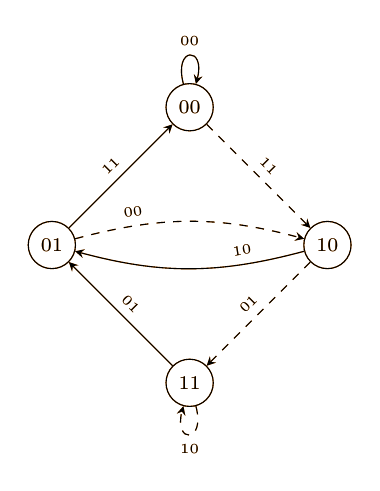
\begin{tikzpicture}[scale=.70, >=stealth, font=\tiny]
\tikzstyle{state} = [draw, circle, inner sep=1mm, minimum size=6mm, font=\scriptsize]
 \alt<2> {\node[state, orange] (state0) at (0,2.5) {00};}{\node[state] (state0) at (0,2.5) {00};}; \alt<3,5> {\node[state, orange] (state2) at (2.5,1.53075794227797e-16) {10};}{\node[state] (state2) at (2.5,1.53075794227797e-16) {10};}; \alt<0> {\node[state, orange] (state3) at (3.06151588455594e-16,-2.5) {11};}{\node[state] (state3) at (3.06151588455594e-16,-2.5) {11};}; \alt<4,6> {\node[state, orange] (state1) at (-2.5,-4.59227382683391e-16) {01};}{\node[state] (state1) at (-2.5,-4.59227382683391e-16) {01};}; \alt<0> {\draw[->, orange] (state0) to [looseness=8,out=105,in=75] node [sloped, above] {00} (state0) ;}{\draw[->] (state0) to [looseness=8,out=105,in=75] node [sloped, above] {00} (state0) ;}; \alt<2> {\draw[->, dashed, orange] (state0) to  node [sloped, above] {11} (state2) ;}{\draw[->, dashed] (state0) to  node [sloped, above] {11} (state2) ;}; \alt<6> {\draw[->, orange] (state1) to  node [sloped, above] {11} (state0) ;}{\draw[->] (state1) to  node [sloped, above] {11} (state0) ;}; \alt<4> {\draw[->, dashed, orange] (state1) to [bend left=15] node [sloped, above,near start] {00} (state2) ;}{\draw[->, dashed] (state1) to [bend left=15] node [sloped, above,near start] {00} (state2) ;}; \alt<3,5> {\draw[->, orange] (state2) to [bend left=15] node [sloped, above,near start] {10} (state1) ;}{\draw[->] (state2) to [bend left=15] node [sloped, above,near start] {10} (state1) ;}; \alt<0> {\draw[->, dashed, orange] (state2) to  node [sloped, above] {01} (state3) ;}{\draw[->, dashed] (state2) to  node [sloped, above] {01} (state3) ;}; \alt<0> {\draw[->, orange] (state3) to  node [sloped, above] {01} (state1) ;}{\draw[->] (state3) to  node [sloped, above] {01} (state1) ;}; \alt<0> {\draw[->, dashed, orange] (state3) to [looseness=8,out=285,in=255] node [sloped, below] {10} (state3) ;}{\draw[->, dashed] (state3) to [looseness=8,out=285,in=255] node [sloped, below] {10} (state3) ;};
\end{tikzpicture}
\end{center}
\end{minipage}
\end{center}

\end{frame}
